\section{Results}
\label{sec:results}

\subsection{First Experiment}

The results of the first experiment are shown in \figref{renaming}. The first important thing to notice is that most of the periods contain only a low amount of renaming. Also, the amount of renaming vary between projects. For instance Jenkins contain only a tiny amount of renaming while PHPUnit have two periods out of four with more than $50\%$ of files renamed. Additionally, the amount of renaming varies drastically among the periods of a same project. For instance in PHPUnit the period 3.6 - 3.7 has less than $5\%$ of files renamed while the period  3.7 - 4.0 has almost $99\%$ of files renamed. We can also notice that initial periods (the leftmost bars in \figref{renaming}) contain usually the bigger amount of renaming (except for PHPUnit). A final interesting finding in this experiment is that major periods do not contain necessarily more renaming than minor periods. For instance in JQuery the period 1.1 - 1.2 has more renaming than 1.9 - 2.0. However, major periods seems to often contain more renaming than minor ones: it is the case in Rails and PHPUnit, while Jenkins and Pyramid contain no major periods.

\begin{figure*}[t]
	\centering
	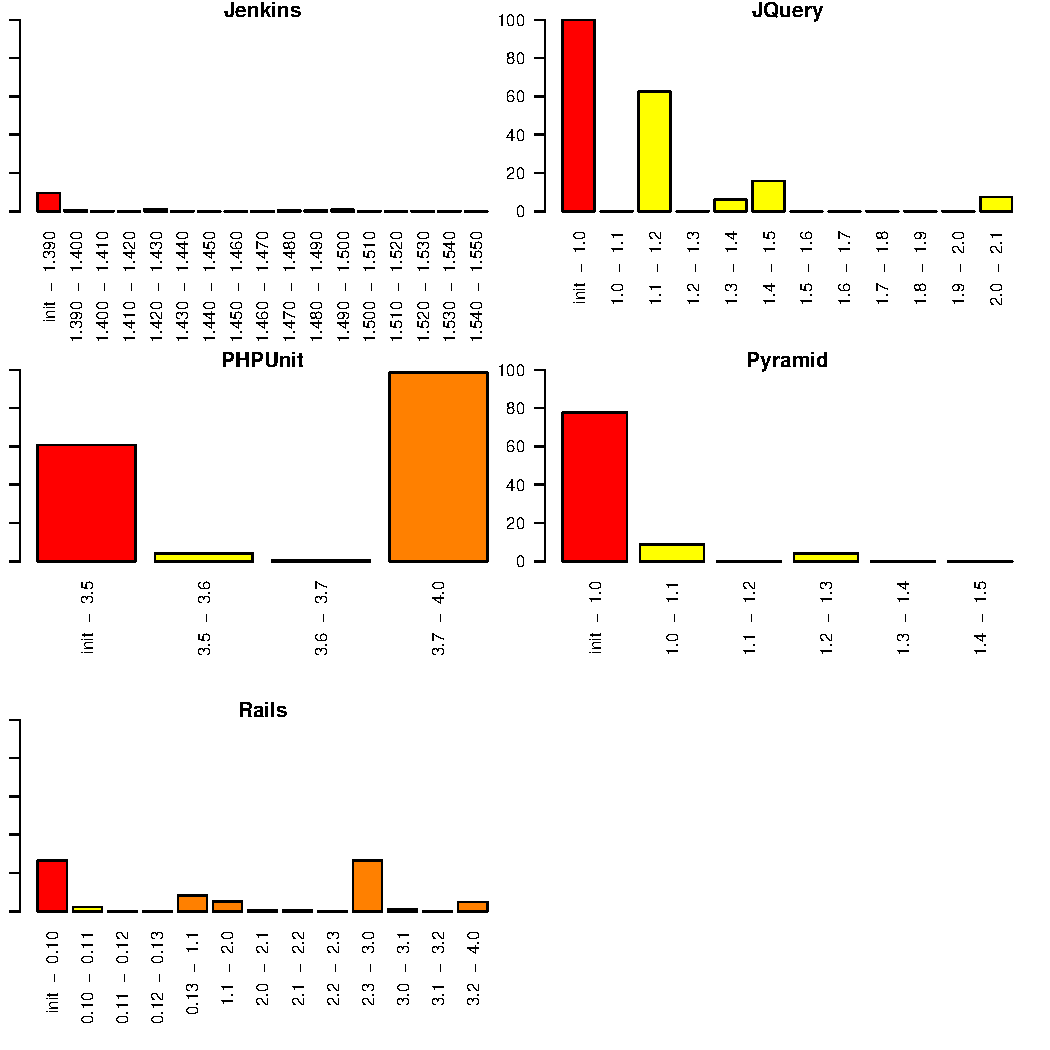
\includegraphics[width=0.85\linewidth,keepaspectratio]{data/figures/renaming.pdf}
	\caption{Percentage of files renamed ($\%F_R$) in each period of each project of our corpus. The initial period is in dark grey, major periods are in medium grey and minor periods are in light grey.}
	\label{fig:renaming}
\end{figure*}

\subsection{Second Experiment}

The results of the second experiment are shown in \tabref{spearman}. It shows that the Spearman correlation coefficients between the metrics with and without renaming highly depend on the considered period and metric. Change metrics of the Jenkins, Pyramid and Rails projects are not affected by renaming as correlation coefficients are close to $1$ in every case. On the other hand, change metrics for the PHPUnit and JQuery projects can be severely impacted by renaming. On JQuery, the CC metric is resilient to renaming, but NoD and NoC are significantly impacted. On PHPUnit, all the metrics are significantly impacted by renaming. On these two projects, the metric more sensible to renaming is number of developers. In this case, it could seriously invalidate the result of a study using these metrics. Finally, we can notice that only the periods having a very high percentage of files renamed ($\%F_R$) are impacted by renaming. We can also notice that skewed change metrics were obtained in both minor and major periods.

We manually investigated the two periods that have significantly skewed change metrics values (JQuery 1.1 - 1.2 and PHPUnit 3.7 - 4.0) to understand why it happened. We remarked that in both periods, the projects directory structures were significantly modified, with several top-level directories that changed names. Therefore a very high number of files were finally transitively renamed. This is not an unusual practice, so this phenomenon might appear in any period of any project. It is interesting to remark that in both periods, this change of structure was performed in only one commit very close to the end of the period.

\begin{table*}[t]
\centering
\small
\csvreader[tabular=rcccc, table head=\toprule & & \multicolumn{3}{c}{Change metrics}\\\cmidrule{3-5} Period & $\%F_R$ & CC & NoD & NoC\\\midrule, late after line=\\, late after last line=\\\bottomrule]{data/tables/correlations.csv}%
{1=\period,2=\fr,3=\churnall,4=\devall,5=\modificationsall}%
{\period & \fr & \churnall & \devall & \modificationsall}
\caption{Spearman correlation coefficients between values of change metrics with and without renaming. The significance codes are: *** $\leq 0.01$, ** $\leq 0.05$, * $\leq 0.1$ and ! $> 0.1$. Medium and low correlation coefficients are displayed in bold.}
\label{tab:spearman}
\end{table*}

\subsection{Threats to Validity}
\label{sec:threats}

Our study makes the assumption that renamed files detected by Git tool are correct. However, we did not encounter any empirical evaluation of the Git renaming detection algorithm and therefore we have no confidence on its results. To mitigate this threat, we drew at random $100$ renamed files detected by Git in our corpus. We manually assessed each detected file renaming to check if it was correctly detected. Checking if a detected file renaming is correct consists in ensuring that the file content is very similar, and that no other file added in the same version has a similar content. This manual analysis revealed that $100\%$ of the detected renamed files were correctly detected. Even though we are aware that Git algorithm can yield false positives, this experiment shows that using Git as an oracle to detect renaming is reasonable. We did not analyzed the false negatives (true file renaming not detected by Git) as this is not a threat to our conclusion, since it will most likely lower the correlation coefficients if underestimated.

Due to a very small number of files, significance values of the correlation coefficients for the JQuery project are low for NoD and NoC. Nevertheless, significance of the correlation is not a threat with regard to our conclusion.

We only assessed the effect of renaming on three change metrics. The effect of renaming could be different (worse or better) for other change metrics. To mitigate this risk we used the most used change metrics as shown in~~\cite{radjenovic_software_2013}. Other change metrics are often based upon these metrics (such as \emph{code ownership}~\cite{bird_dont_2011} or \emph{module activity focus}~\cite{posnett_dual_2013}).

For the NoD metric, we did not apply an identity merging algorithm~\cite{goeminne_comparison_2013}. This could result in incorrect values. However, this phenomenon is likely to happen for both metrics with and without renaming, therefore the risk that it invalidates our conclusion is low.

Concerning our conclusion on the amount of renaming, the corpus we used do not guarantee that it is generalizable. Indeed, we only used open-source projects, while industrial projects are known to be significantly different. Regarding the validity among open-source projects, our corpus is to small to generalize our conclusion.
